\subsection{Interface Requirements}


\subsubsection{User interfaces}
In Figure \ref{fig:user_pm_registration} we can see the registration page. If a Visitor doesn’t already have an account he can decide to create a new one, by inserting all the required data (name, surname, birthday, area of residence, email and password). Policy makers who wants to register, need to click on the “Policy maker” tab and after clicking on it, a new field will appear asking to insert the Policy maker ID.\\
\begin{figure}[h!]
\centering
\begin{subfigure}{.4\textwidth}
  \centering
  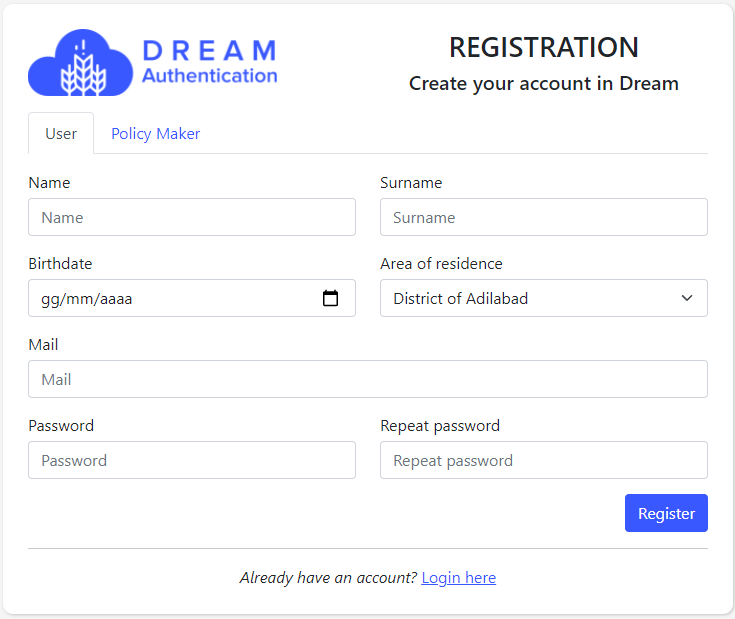
\includegraphics[width=1.075\linewidth]{images/interfaces/register_user.png}
  \caption{User}
  \label{fig:user_registration}
\end{subfigure}\hfill
\begin{subfigure}{.4\textwidth}
  \centering
  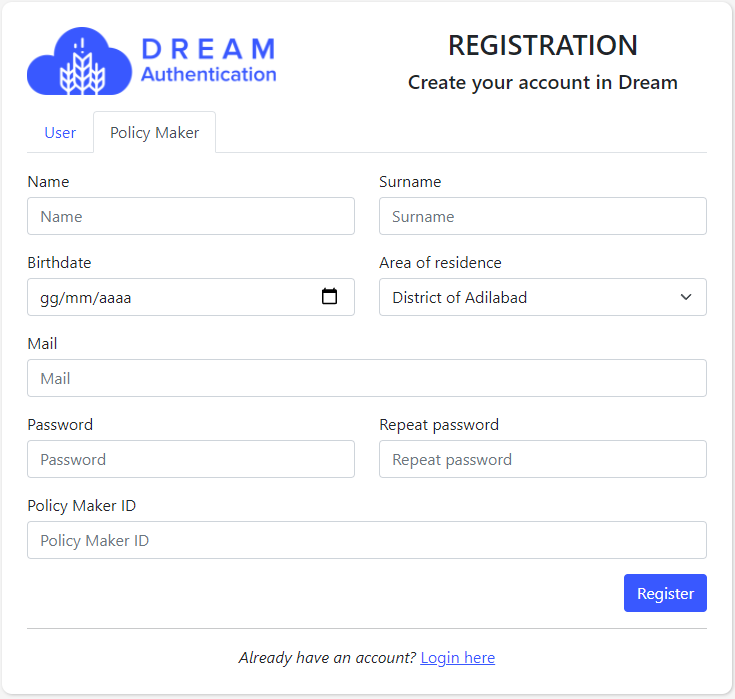
\includegraphics[width=1\linewidth]{images/interfaces/register.png}
  \caption{Policy maker}
  \label{fig:pm_registration}
\end{subfigure}%
\caption{Register pages}
\label{fig:user_pm_registration}
\end{figure}
\FloatBarrier

\subsubsection{Policy maker interfaces}
The Policy maker reserved area interface is composed by two different columns: on the left there is the menu with a list of the different section. Once selected the section of interest, the right part of the page renders the corresponding view.\\ In Figure \ref{fig:deviance_page} we can see the "Deviance" section: a ranking list of areas is represented alongside the checkbox list in which the Policy maker can choose the parameters that will be taken into account when a new Deviance is recalculated.
\begin{figure}[h!]
    \centering
    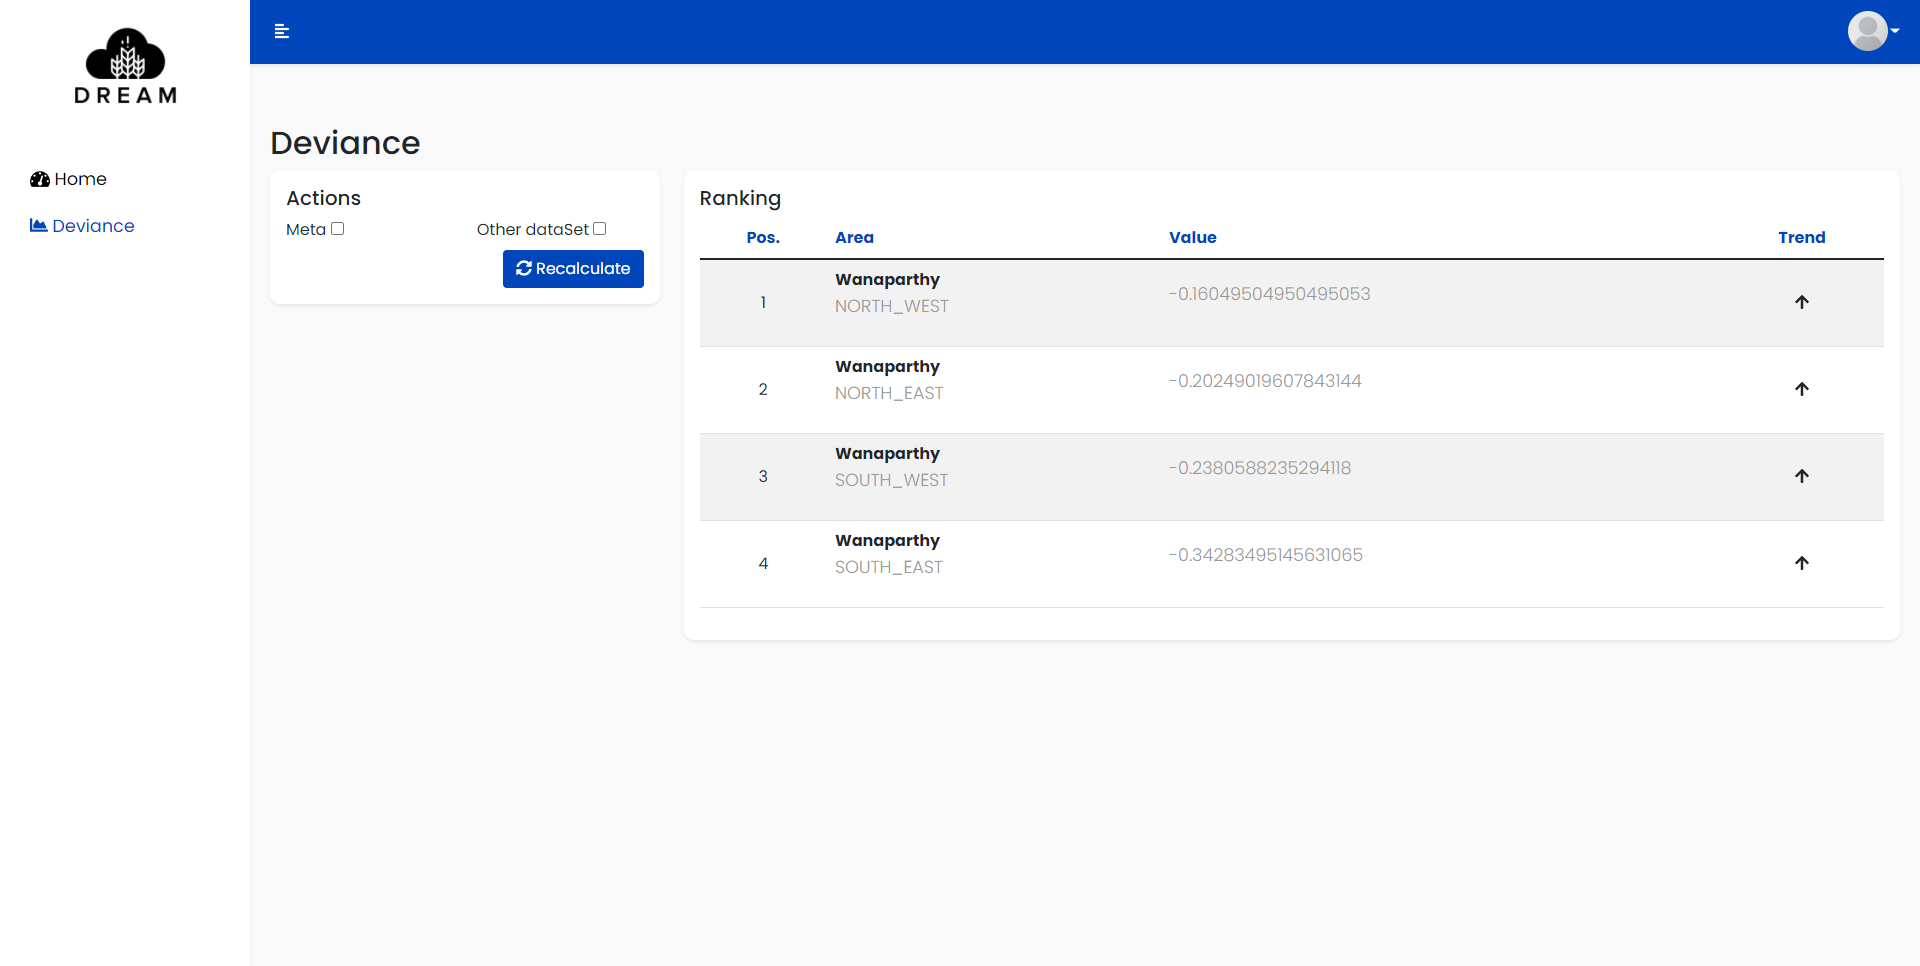
\includegraphics[scale=0.2]{images/interfaces/deviance.png}
    \caption{Deviance page}
    \label{fig:deviance_page}
\end{figure}
\FloatBarrier

\subsubsection{Administrator interfaces}
The Administrator reserved area (Figure \ref{fig:datasources}) interface is composed by two different columns: on the left there is the menu with the list of the different sections (similar to the Policy makers' one). In this case the "Data Sources" page is selected and a table with all the active sources in the system is visible. For each row two buttons are available: the first one is a gear and it is used to display the configuration of the corresponding data source, while the second one, is a red trash bin and if it's clicked it lets the Administrator to delete the corresponding data source. Finally on the top right part of the internal view there is a button that lets the Administrator to add a new data source.  
\begin{figure}[h!]
    \centering
    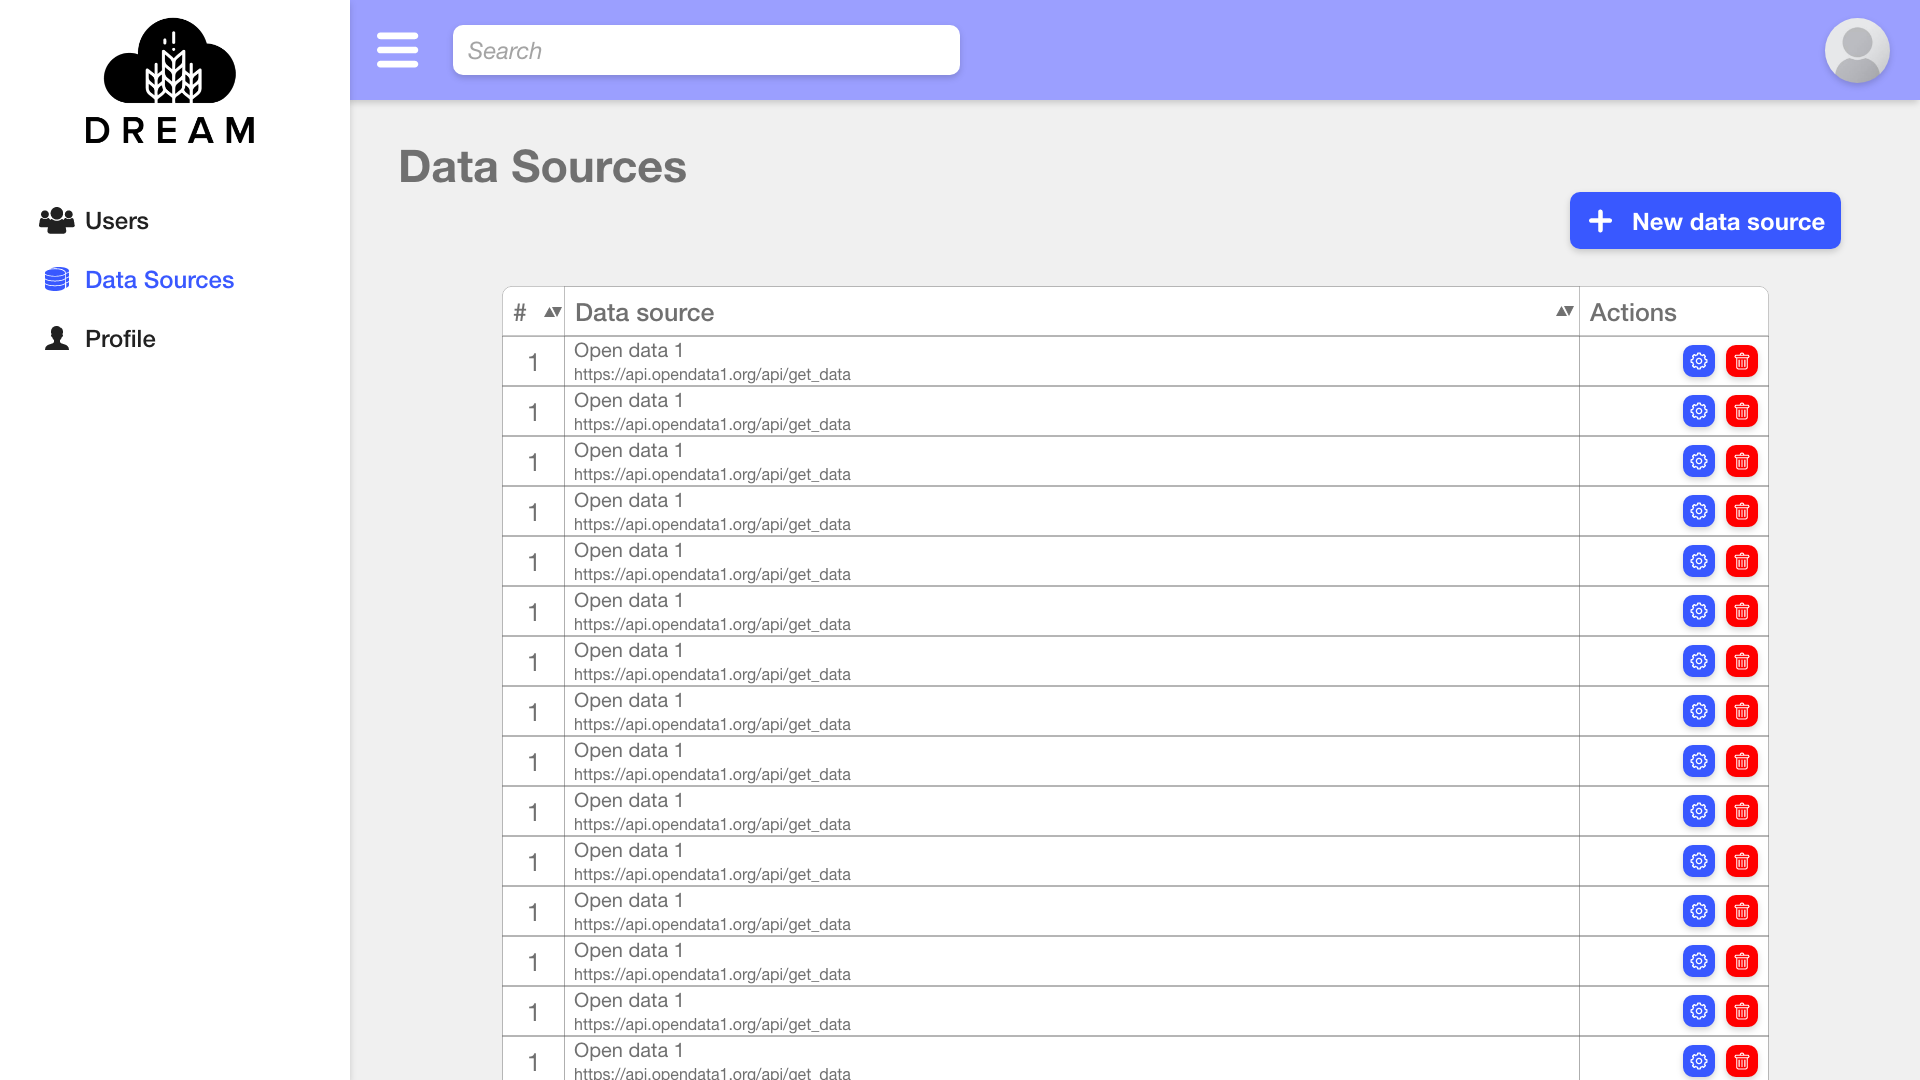
\includegraphics[scale=0.2]{images/interfaces/data_sources.png}
    \caption{Data sources}
    \label{fig:datasources}
\end{figure}
\FloatBarrier
\subsubsection{Forum interfaces}
The Forum’s home page is like in Figure \ref{fig:forum_home} and it’s divided in three columns. The first one represents the menu, in which it’s presents the “Home” tab (containing a list of all the topics) and the “Explore topics” tab (containing random discussion belonging to different topics).
Since in the figure it’s selected the “Home” tab, we can see in the central column a list of all the topics present in the forum. Finally, in the third column are present two boxes: the first one contains a list of the most active User and the second one holds different quick links.
Clicking a topic, we will be redirected to a new page containing a list of all the discussion contained in the selected topic (Figure \ref{fig:forum_discussion}) and clicking on a discussion we will be redirected to the selected one, from which we can also see the complete text of the discussion and all its replies (Figure \ref{fig:forum_post}).
\begin{figure}[h!]
    \centering
    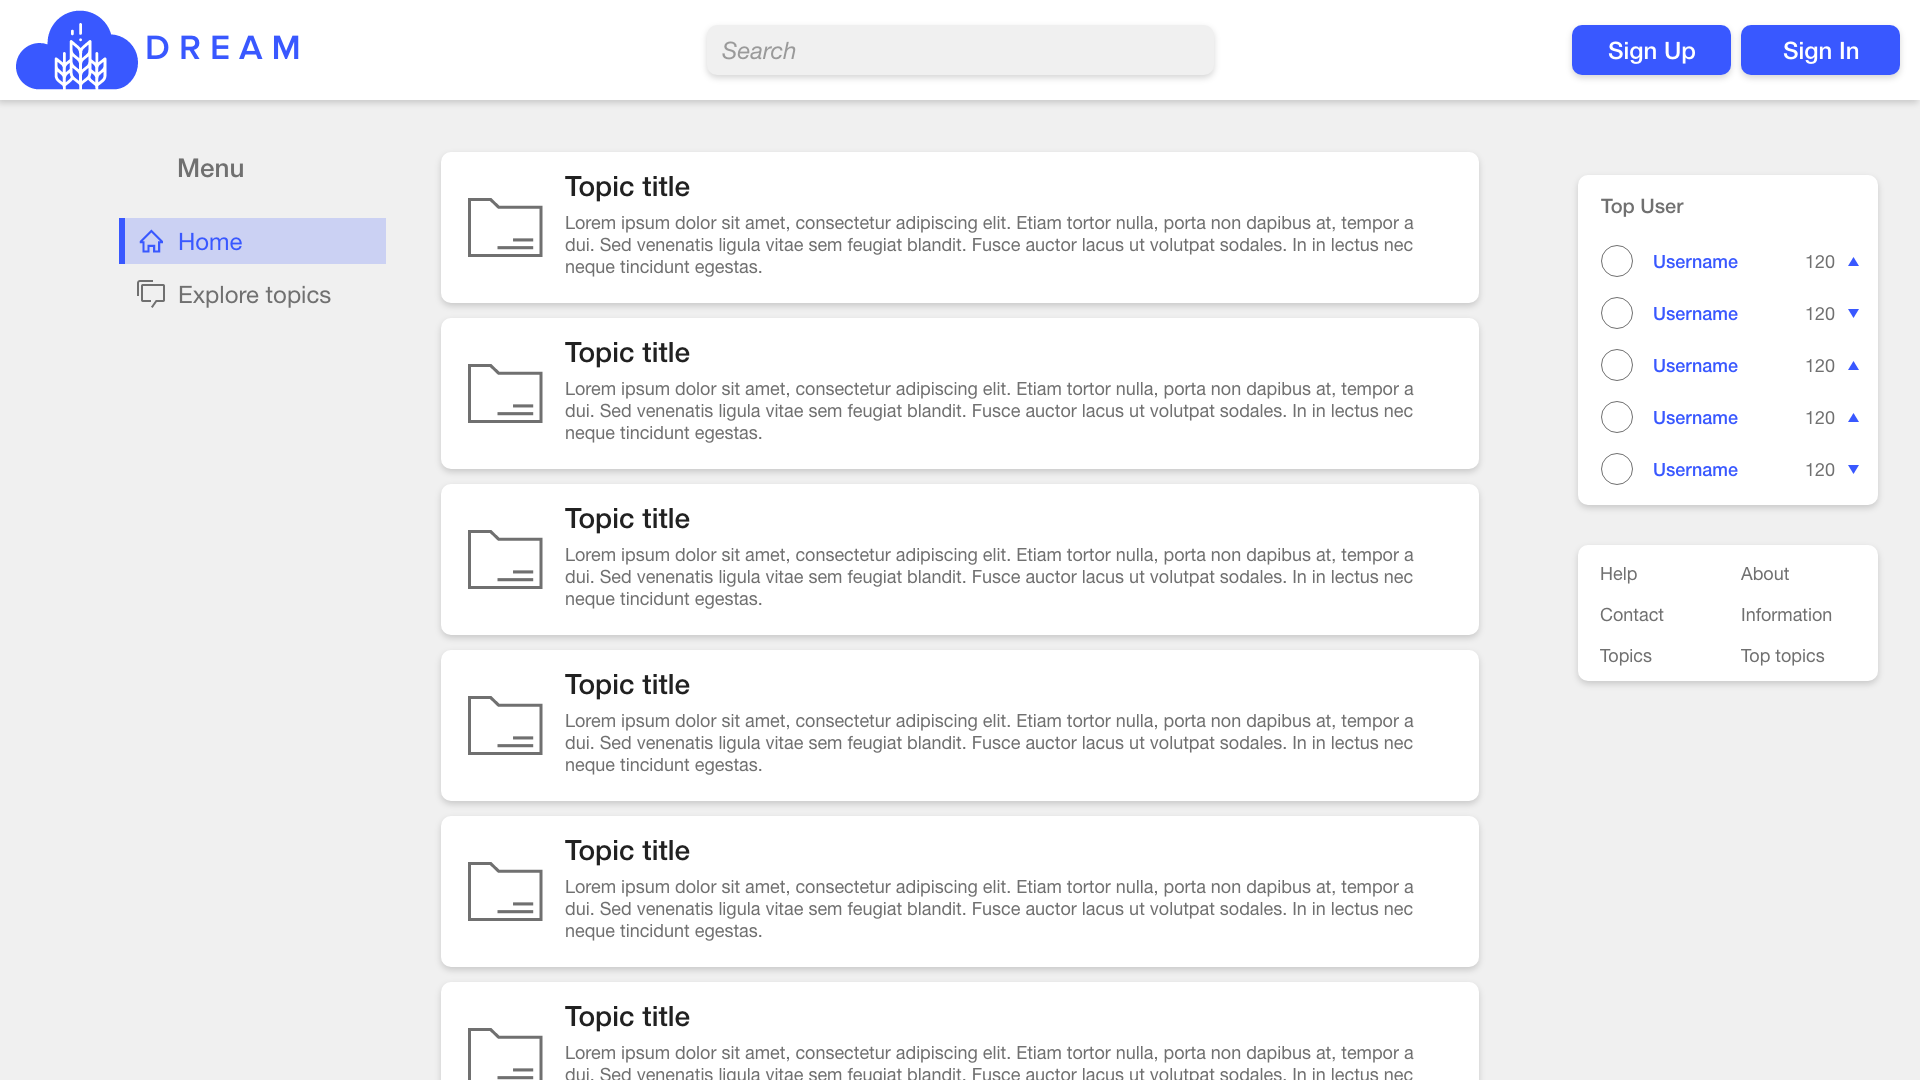
\includegraphics[scale=0.2]{images/interfaces/forum_topic.png}
    \caption{Forum homepage (without login)}
    \label{fig:forum_home}
\end{figure}
\begin{figure}[h!]
    \centering
    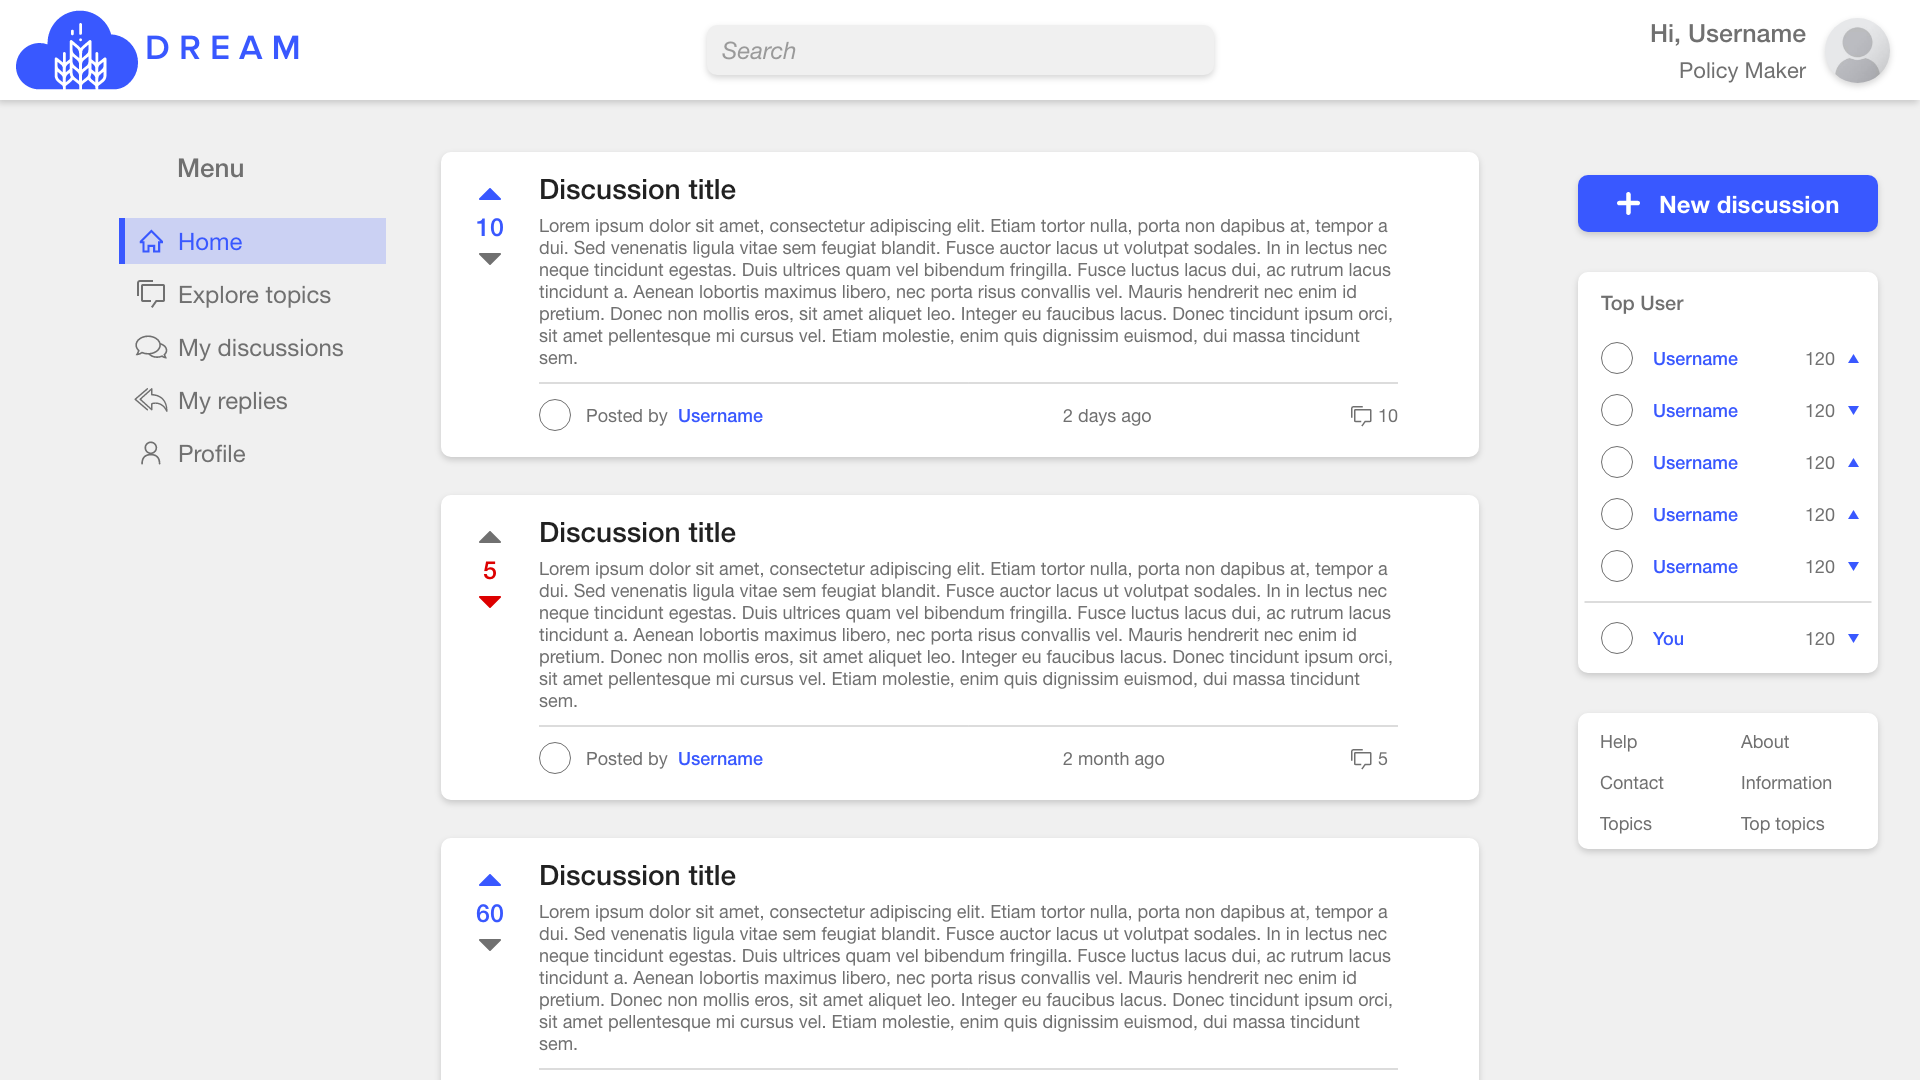
\includegraphics[scale=0.2]{images/interfaces/list_discussion.png}
    \caption{Discussions inside a topic}
    \label{fig:forum_discussion}
\end{figure}
\begin{figure}[h!]
    \centering
    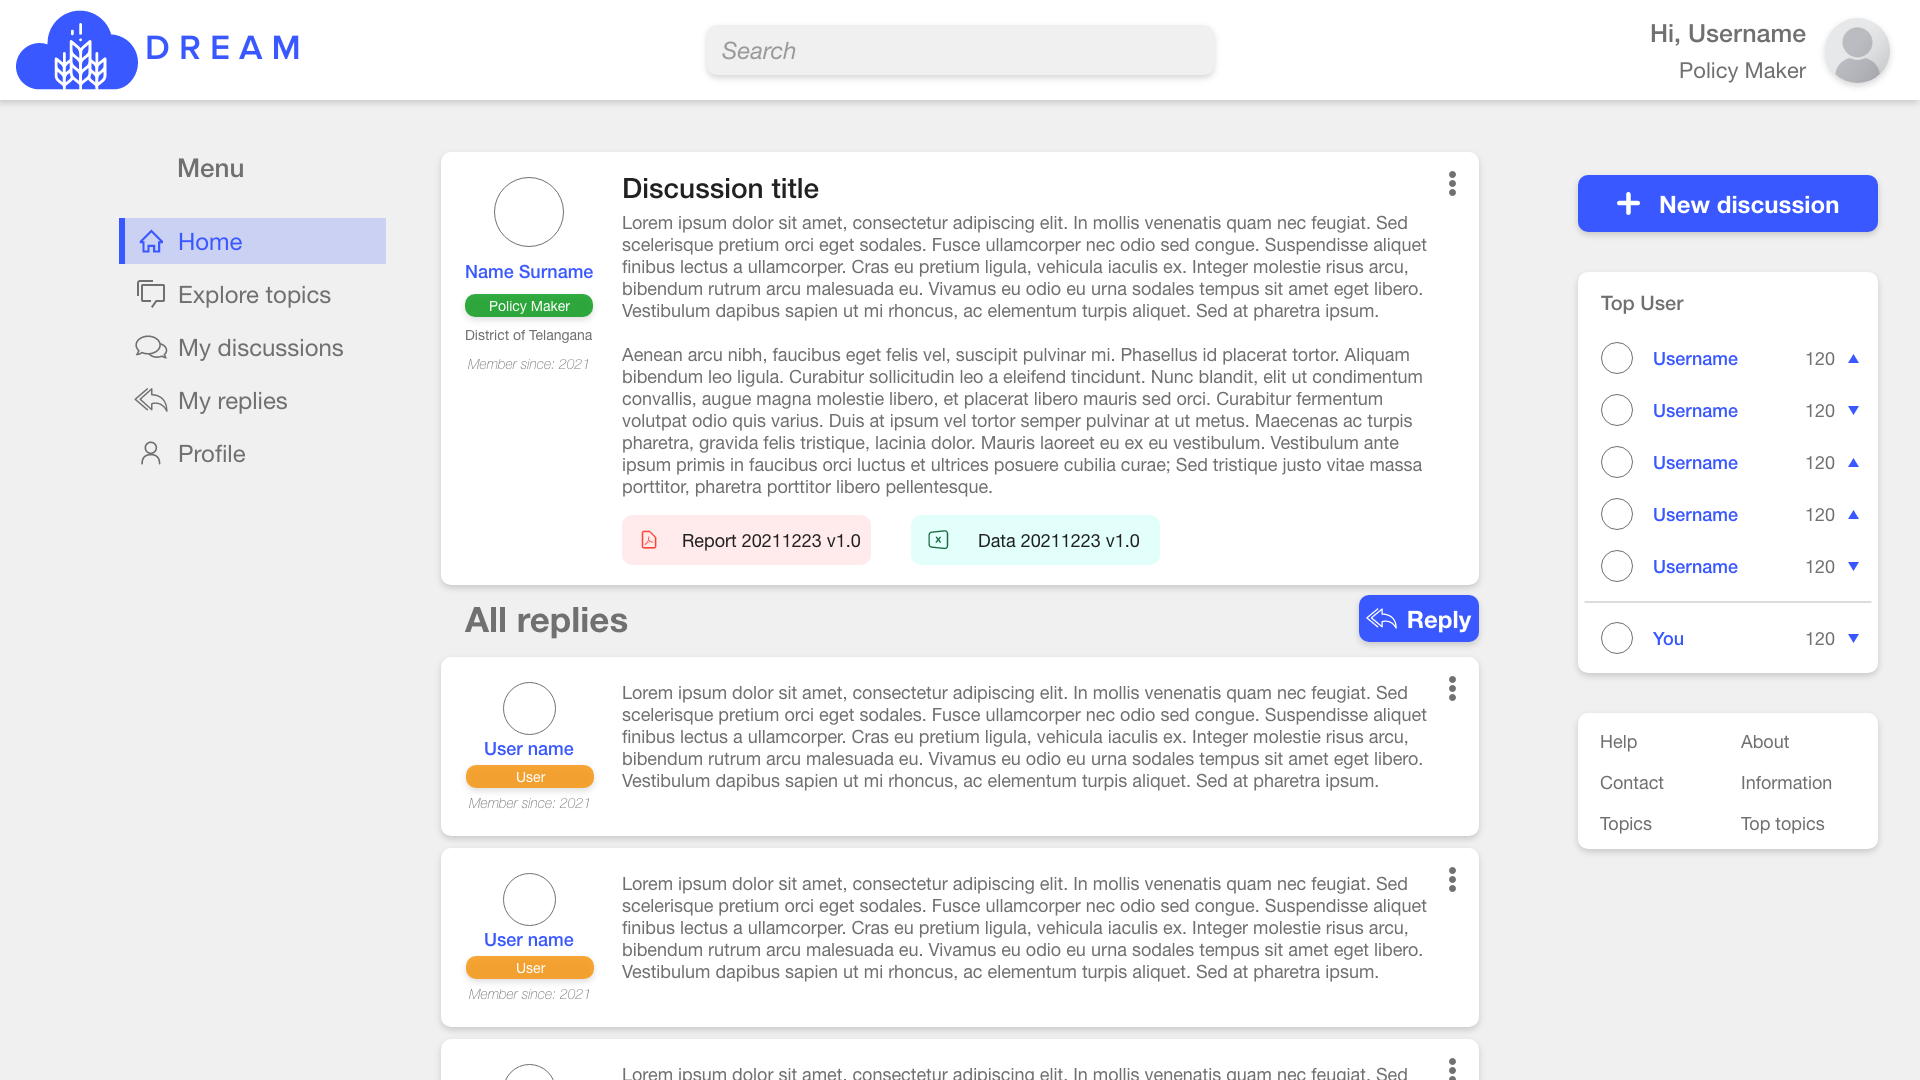
\includegraphics[scale=0.2]{images/interfaces/discussion.png}
    \caption{Content of a discussion}
    \label{fig:forum_post}
\end{figure}
\FloatBarrier
\subsubsection{Homepage interface}
We can also see in Figure \ref{fig:homepage} the home page of the site, where the Visitor could access the data or Sign up/Sign in. In this page, if a Policy maker is already logged in, it's present a button from which the Policy maker can reach his Reserved Area.
\begin{figure}[h!]
    \centering
    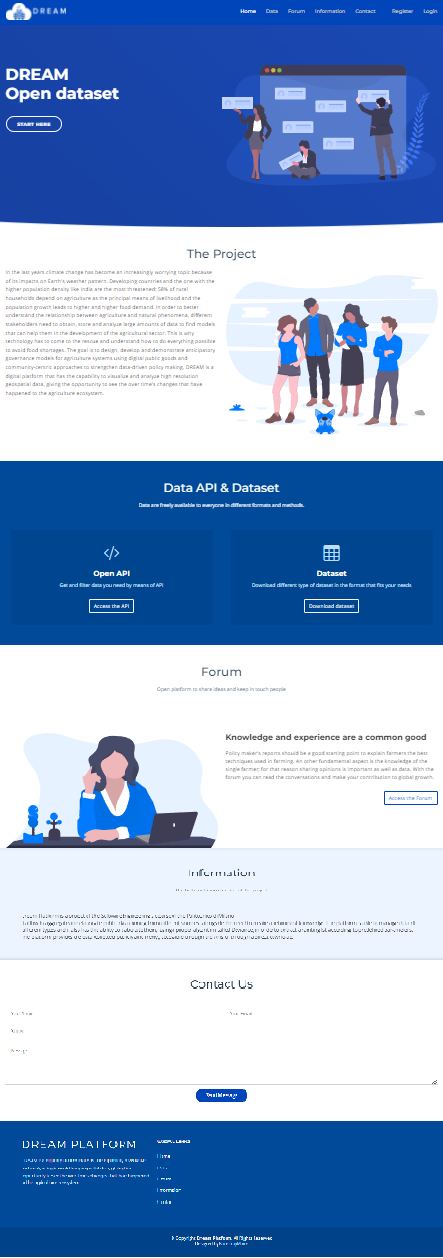
\includegraphics[scale=0.55]{images/interfaces/home.png}
    \caption{DREAM Homepage}
    \label{fig:homepage}
\end{figure}
\FloatBarrier
